\chapter{Empirical Experiments}\label{chapter:experiments}
% \setcounter{page}{0}
% \pagenumbering{arabic}

\section{Prices and Filling Information}
To have a comprehensive understanding of how trades in trade book correspond to orders in order book, Figure~\ref{fig:p_f_i} provides an overview of the whole active trading hours from 10:00 am to 4:00 pm on 31st January. It shows how filled price in the trade book track the mid-price in the order book, the distribution of passive and aggressive trades, and the spread range for each trade. The lower subplot presents the filled volume for each trading record.
\begin{figure}[h]
    \centering
    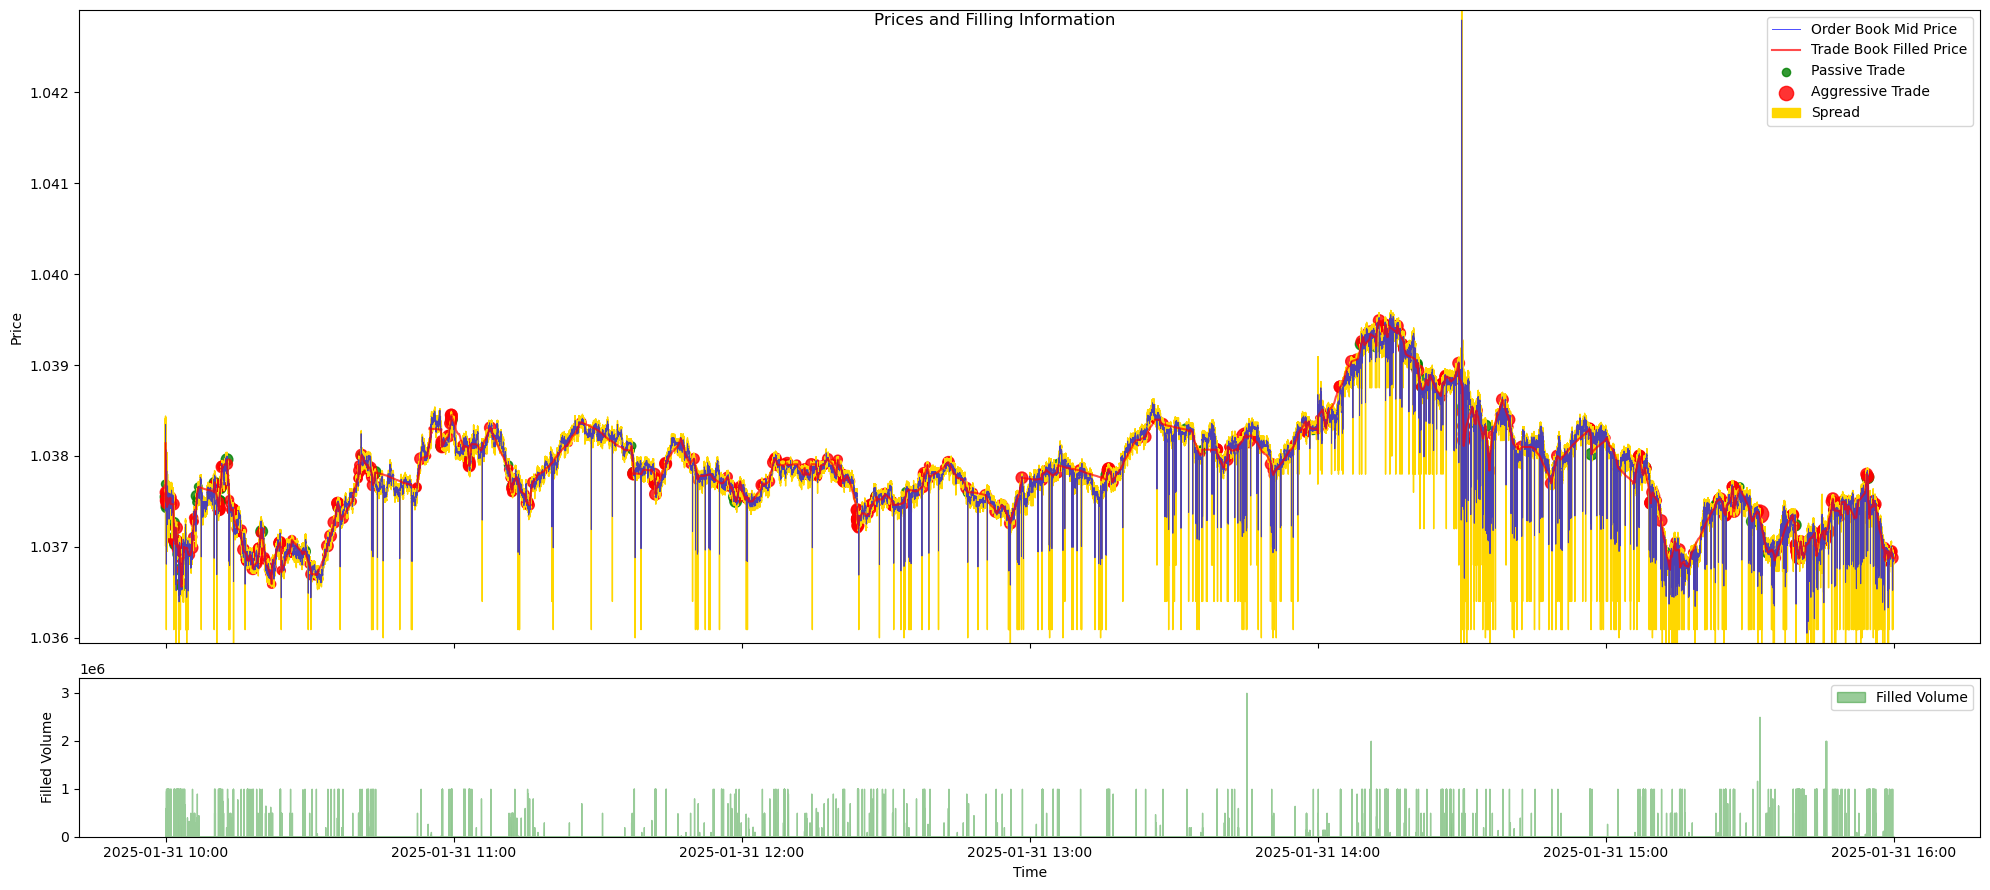
\includegraphics[width=1\linewidth]{figures/Prices and Filling Information.png}
    \caption{Prices and filling information. This plot shows the mid-price from the order book (blue line), trade book filled prices (red line), and spread (yellow shading). Passive trades (green dots) and aggressive trades (red dots) are highlighted. The bottom panel represents the filled volume over time.}
    \label{fig:p_f_i}
\end{figure}
As can be seen in Figure~\ref{fig:p_f_i}, the mid-price has the highest point between 14:00 and 15:00. The filled price fits the mid-price well. We can see there are a lot of red dots which shows that they are aggressive trades. We didn't classify bid or ask side because it's not the research target in the thesis. These aggressive trades go outside the spread range. The size of dots stands for relative volume of the trades. In other words, when the volume is large compared to other timestamps, the size of the dot will be larger. Therefore, we can easily see the active trading time point in the plot. Moreover, red dots represent aggressive trades in the trade book. We can see the red dots are more than green ones, which indicates that a lot of orders get filled by aggressive traders taking out them of the order book, instead of passively waiting for the market movements. This aligns with our need to improve the backtesting environment by predicting aggressive trades across the order book. Specially, there are several sparks in the trend of mid-price in the order book. These are caused by...

From the bottom panel, in the beginning of 10:00, 15:45, 14:11, there are high volume up to 2,000,000, which are higher than common volume 1,000,000. At 13:45, the highest trading volume occurs as 3,000,000. Combined the two plots together, we can see when there's a drop, it's often accompanied by many trading records or large trades. 

\begin{figure}[h]
    \centering
    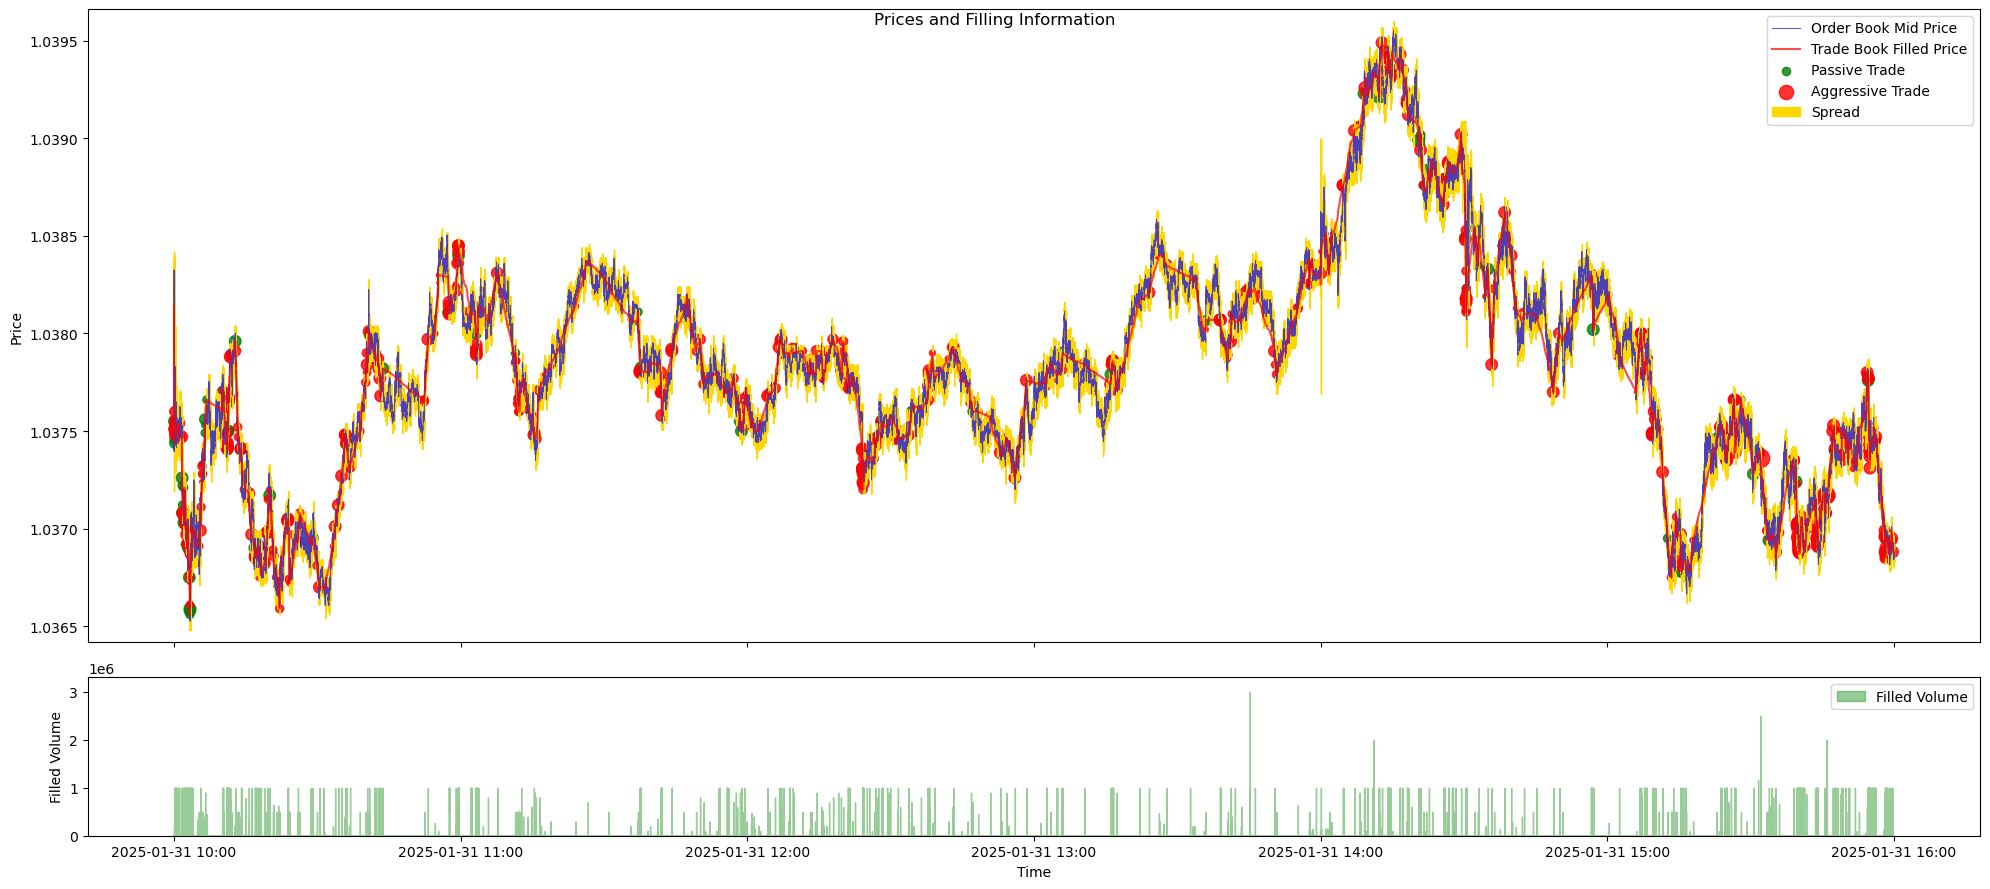
\includegraphics[width=1\linewidth]{figures/Filtered Prices and Filling Information.png}
    \caption{Filtered prices and filling information. Similar to Figure~\ref{fig:p_f_i}, but filtering sharp jump points. The price and trade dynamics remain the same, without increased variability for better general trend capture}
    \label{fig:f_p_f_i}
\end{figure}

In the Figure~\ref{fig:f_p_f_i} after filtering 1,232 sparks in the data, we can clearly see some clustering for both passive and aggressive trades. For example, in the beginning of 10:00, many passive trades gather here. It may because there's a sharp dropping movement in the market, many limit orders are filled. Furthermore, many aggressive trades gather around  


% Evaluating how well the model captures aggressive trades movements and distribution.
% Market realism (stylized facts: price impact, spread, volume clustering).

\section{Prediction Results}
The prediction framework consists of three sequential stages. The first stage employs an XGBoost model to identify potential aggressive trade timestamps while reducing the overall dataset size. The second stage is GRU networks. It serves as a bridge between machine learning approaches and stochastic processes. It generates hidden states as neural kernels. The final stage implements a neural Hawkes process that estimates event intensity. In the end this approach produces a detailed and interpretable decision of predictions for aggressive trading events.

We present the prediction results of each stage using a representative trading day. The training dataset consists of the whole trading day from January 31, 2025, 10:00:00 to 15:59:59 PM, containing 307,764 rows. This day is chosen because it contains lots of market information and trade data, which is the most comprehensive trading day across the whole dataset. 

The testing datasets are some 30-minute, 1-hour windows from different trading days, each with around 20,000 rows. This specific time window was selected as it represents a commonly used timeframe for FX trading backtesting within the MN platform.

\subsection{XGBoost Stage: With and Without KMeansSMOTE}

KMeansSMOTE, introduced in Chapter~\ref{chapter:methodology}, is an oversampling technique designed to address class imbalance in training data. We compare the XGBoost prediction results with and without KMeansSMOTE to evaluate the influence of oversampling. The impact of applying this oversampling method on both class balance and prediction quality is analyzed.

We first present the classification results of XGBoost trained with KMeansSMOTE. The KMeansSMOTE configuration is as follows:

\begin{verbatim}
pipeline = Pipeline([
("imputer", SimpleImputer(strategy="median")),
("smote", KMeansSMOTE(random_state=42,
cluster_balance_threshold=0.02,
kmeans_estimator=KMeans(n_clusters=200, random_state=42),
sampling_strategy=0.5))
])
\end{verbatim}

The median strategy fills missing values with the median of each feature. A cluster balance threshold of 0.02 ensures oversampling is done in 'safe' areas where there are at least some genuine minority examples. As a result, the training set has the ratio of 3:7 about class 1 and class 0. It significantly increases the class balance from 1:499 in Figure~\ref{fig: aflag_class_distribution}.

This step is aimed to get a model to initially find out as many positives as possible by keeping recall as 0.6 without losing precision. So, the input for testing only depends on market features ($S$, $M$, $V_A^{1}$, $V_A^{1}$, $\bar{\delta}_S$, $\bar{\delta}_M$, $\sigma_S$, $\sigma_M$, $r_V$), and the output contains the shortened training dataset for the next step with aggressive trade candidates. The filtered output also gets rebalanced towards class 1 because we filter out those are not predicted as 1. the bias toward class 0 and helps the model learn better from the underrepresented class 1.

As shown in Figure~\ref{fig:xgb-pred-vs-true-km}, the model catches many true positives. The class balancing done by KMeansSMOTE reduces the bias toward class 0 and helps the model learn better from the underrepresented class 1.

Table~\ref{tab:xgb-confusion-km} shows the confusion matrix. 4,011 are predicted as class 0 (non-aggressive trade), and 3,739 are predicted as class 1. The model correctly finds 13 true positives and 4,001 true negatives. The dataset size drops from 7,750 to 3,739 rows, which is 51.75\% of the original. This helps improve speed and keeps most of the important trade points.

Moreover, Table~\ref{tab:xgb-classification-report-km} shows the detailed classification report. We mainly care about the prediction performance for class 1, since this is the main goal of the whole research. The precision of class 0 is not meaningful here because the original data is extremely imbalanced. Although the precision for class 1 is still very low at 0.0035, the recall reaches 0.5652. This means the model finds sufficient true trades under the model with oversampling. This makes preparation for next neural Hawkes process.


\begin{figure}[H]
    \centering
    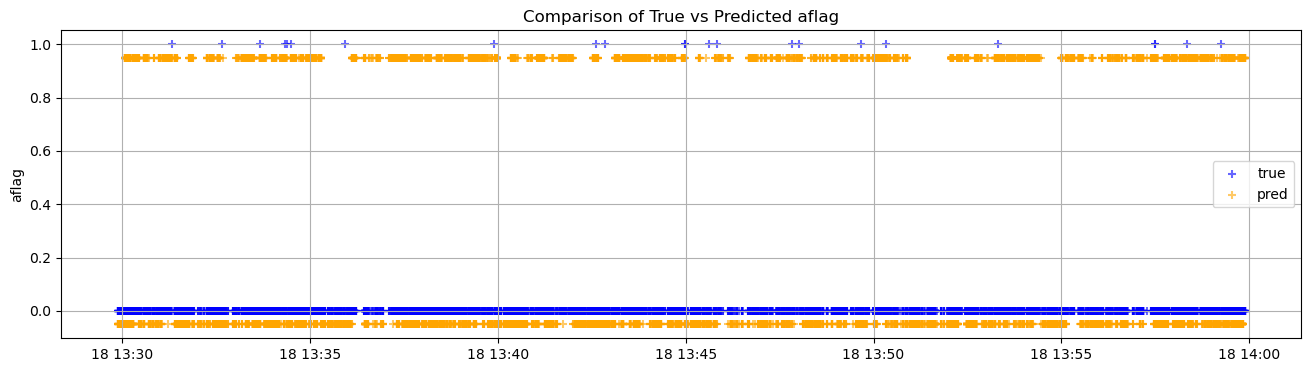
\includegraphics[width=\textwidth]{figures/aflag_XGBoost_181330.png}
    \caption{Comparison of true vs. predicted $\bar{\alpha}$ from XGBoost with KMeansSMOTE. 
    The blue '+' markers show the true class labels, and the orange '+' markers show the predicted ones. To make the plot easier to read, the predicted values are moved down by 0.05 on the y-axis. This small shift helps to see clearly how well the predictions match the true labels.
    }
    \label{fig:xgb-pred-vs-true-km}
\end{figure}

\begin{table}[H]
    \centering
    \caption{Confusion matrix of XGBoost with KMeansSMOTE}
    \label{tab:xgb-confusion-km}
    \begin{tabular}{lcc}
        \toprule
        & Predicted 0 & Predicted 1 \\
        \midrule
        True 0 & 4,001 & 3,726 \\
        True 1 & 10 & 13 \\
        \bottomrule
    \end{tabular}
\end{table}
\begin{table}[H]
    \centering
    \caption{Classification report of XGBoost with KMeansSMOTE}
    \label{tab:xgb-classification-report-km}
    \begin{tabular}{lcccc}
        \toprule
        Class & Precision & Recall & F1-score & Support \\
        \midrule
        0 & 0.9962 & 0.5178 & 0.6817 & 7727 \\
        1 & 0.0035 & 0.5652 & 0.0069 & 23 \\
        \midrule
        Accuracy & \multicolumn{4}{c}{0.5179} \\
        \bottomrule
    \end{tabular}
\end{table}

Without KMeansSMOTE, even if we reach the same recall, the precision is even worse (only 0.0019). That means almost all predicted class 1 are wrong. The F1-score is just 0.0038, which is only half of the score from XGBoost with KMeansSMOTE. Also, the filter effect is weaker. More lines (5,065) are left in the result, which makes the next detection step slower and more difficult. So using KMeansSMOTE helps not only improve model performance but also makes the pipeline more efficient.

\begin{table}[H]
    \centering
    \caption{Confusion matrix of XGBoost without KMeansSMOTE}
    \label{tab:xgb-noKM}
    \begin{tabular}{lccc}
        \toprule
        Class & Precision & Recall & F1-score\\
        \midrule
        1 & 0.0019 & 0.5881 & 0.0038 \\        
        \bottomrule
    \end{tabular}
\end{table}

These results show that KMeansSMOTE gives significant improvement when dealing with extreme class imbalance, especially in terms of F1-score. We can also infer from the classification evaluation that single XGBoost is not enough for the prediction task even with resampling methods. The large set of candidate points predicted at this stage will be passed to the next neural Hawkes model, which helps to further clean and refine the aggressive trade signals. 


%------------- Neural Hawkes process -------------
\subsection{Neural Hawkes Process Results}
We use the GRU model as a neural kernel to generate hidden states, which are then used in the Hawkes process. The estimation is performed on the dataset from January 31, 2025, between 10:00:00 and 15:59:59. This period is the same as the XGBoost training set, but the data is filtered using the anomaly detection function in Algorithm~\ref{al: window-based} to solve class imbalance.

In the estimation stage, the GRU is already trained and hidden states \( h_t \) are extracted. These hidden states are injected into the Hawkes intensity formula as in Equation~\ref{eq:intensity}. We estimate the parameters by minimizing the negative log-likelihood using the L-BFGS-B method. The optimization process completed in 363.98 seconds, with the final negative log-likelihood reaching $-8261.28$, and success flag returned as \texttt{True}.

\vspace{1em}
\noindent\textbf{Estimated Parameters:}
\begin{itemize}
    \item \textbf{Baseline intensity} (\( \mu \)): [0.0677, 0.0029] \\
    This means, without any past event influence, the natural (background) chance of non-aggressive trade is higher than aggressive trade.
    
    \item \textbf{Excitation matrix} (\( \alpha \)): 
    \[
    \begin{bmatrix}
    10.12 & 15.85 \\
    0.52 & 2.57
    \end{bmatrix}
    \]
    The top row shows how past events of both types excite type 0 (non-aggressive), and the bottom row shows how they excite type 1 (aggressive). An aggressive trade (type 1) causes a strong self-excitation (2.57), but has much smaller influence on non-aggressive (0.52). Cross-excitation from aggressive to non-aggressive (15.85) is very high. This also reflects the important clustering property, which will be explained more in detail later.

    \item \textbf{Decay matrix} (\( \beta \)): 
    \[
    \begin{bmatrix}
    10.55 & 18.48 \\
    62.32 & 14.76
    \end{bmatrix}
    \]
    Each value in the decay matrix \( \beta_{kj} \) represents how quickly the effect of a past event of type \( j \) fades when it influences the intensity of type \( k \).\\
    A non-aggressive trade (type 0) decays with a moderate speed when it influences another non-aggressive trade (\( \beta_{00} = 10.55 \)). When an aggressive trade (type 1) influences non-aggressive activity (\( \beta_{01} = 18.48 \)), the effect decays faster, suggesting a short but noticeable reaction from the market. On the other hand, a non-aggressive trade has almost no lasting effect on aggressive trades, as shown by the very fast decay rate (\( \beta_{10} = 62.32 \)). Lastly, the self-decay for aggressive trades (\( \beta_{11} = 14.76 \)) is moderate, meaning aggressive trades may cluster slightly, but the effect also wears off gradually. This is expected, as market reacts quickly after an aggressive trade occurrence.
\end{itemize}

% !!need careful explain of this plot
Figure~\ref{fig:neuralhp-intensity} shows the result of the intensity simulation based on the fitted model and the hidden states from GRU. It is generated by computing the intensity at evenly spaced timestamps over the trading period. The model uses the hidden state \( h_t \) from GRU at each time point, along with the event history up to that point, to calculate the intensity values. 

The top plot shows the total intensity across both types. It has many spikes, showing clustering of trading activity. The small purple markers indicate when actual events occurred. The middle plot shows the intensity for type 0 (non-aggressive). It has strong fluctuations and many large peaks, which align well with the red event markers, meaning the model successfully captures those trades. The bottom plot is for type 1 (aggressive). The intensity is generally much lower, and spikes are fewer. Still, many aggressive trade events align with sharp local peaks. This shows that the model correctly adjusts intensity to reflect aggressive trade likelihood.

\begin{figure}[H]
    \centering
    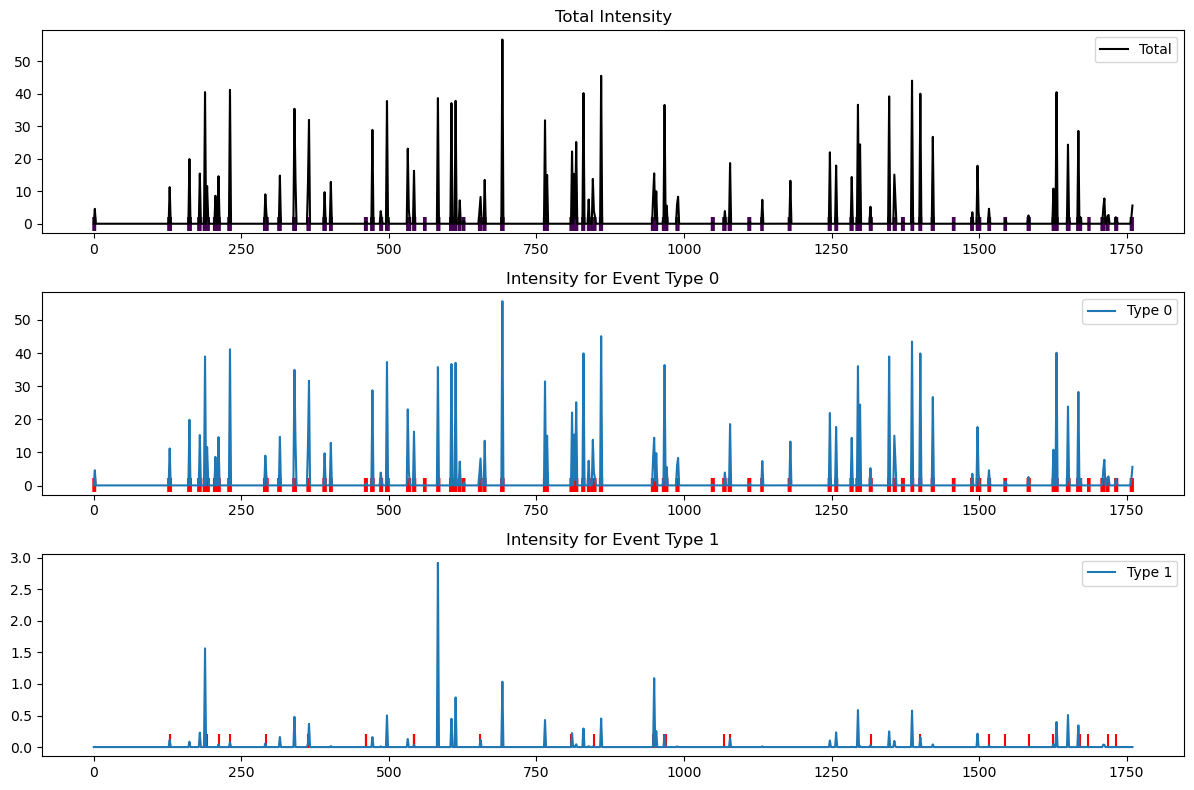
\includegraphics[width=0.95\linewidth]{figures/hp_estimation.png}
    \caption{Estimated intensity functions for each event type. Red markers indicate actual event times.}
    \label{fig:neuralhp-intensity}
\end{figure}

%stop here 6.18 1.28am
%------------ prediction -------------
After getting the estimated parameters from the training phase, we test the Neural Hawkes Process on unseen data. The input for prediction comes from the test output dataset of the XGBoost classifier. This dataset was designed to contain more aggressive trades by predicting as many positives as possible, helping us balance the class better during prediction. It includes market features such as spread ($S$), mid-price ($M$), volume at best ask and bid ($V_A^1$, $V_B^1$), short-term average changes ($\bar{\delta}_S$, $\bar{\delta}_M$), volatilities ($\sigma_S$, $\sigma_M$), and volume ratio ($r_V$). These can all be fetched from Snowflake or calculated by raw data. These features are used to extract hidden states from the GRU, and the corresponding timestamps ($T$) are passed into the Hawkes process to compute event intensities using the previously estimated parameters.

We first conduct prediction on a sample from 2025-02-18 13:30:04.710 to 2025-02-18 13:59:53.060. After getting filtered in XGBoost, which filters as many aggressive trades as possible and helps the model learn more actively from hidden market states, the model predicts 38 points as aggressive trades. In reality, 23 of them are actual aggressive trades. It is acceptable because we are more tolerant to false positives than false negatives.

Exact matching with reality is not good, as the model predicts 38 aggressive trades while only 23 are truly observed. This difference is expected because the neural Hawkes process simulates events based on the fitted intensity, and its goal is to capture realistic patterns, not exact copies of the actual sequence. In the MN backtesting context, capturing similar temporal behaviors and the overall shape of the trade activity is more important than matching every timestamp precisely. Below we explain the evaluation results of each metric shown in Table~\ref{tb:Evaluation Metrics}.


%----------Temporal Alignment---------
The \textbf{Dynamic Time Warping (DTW)} distance is 23.0, with a normalized DTW value of 0.00297. This is very low, which shows that the predicted trade activity follows a very similar time pattern as the actual aggressive trades. The alignment path length is 15464, and the diagonal ratio is 1.995. A ratio close to 2 means the predicted and actual sequences align almost one-to-one. These results confirm that the model learns the shape and rhythm of the trading activity well.
\begin{table}[H]
    \centering
    \caption{Dynamic Time Warping (DTW) Results}
    \label{tb:dtw-results}
    \begin{tabular}{lr}
    \toprule
    Metric & Value \\
    \midrule
    DTW Distance & 23.0 \\
    Normalized DTW Distance & 0.00297 \\
    Alignment Path Length & 15,464 \\
    Diagonal Ratio & 1.995 \\
    \bottomrule
    \end{tabular}
\end{table}

The \textbf{Wasserstein distance} is 0.0019, and the normalized value is also 0.0019 out of a possible maximum distance of 1.0. This is extremely low. It means that the distribution of predicted event times is almost the same as the real distribution. This is a very strong result, showing that even if the model doesn't predict every individual event correctly, the timing and density of trades over time is very accurate.
\begin{table}[H]
    \centering
    \caption{Wasserstein Distance Results}
    \label{tb:wasserstein-results}
    \begin{tabular}{lr}
    \toprule
    Metric & Value \\
    \midrule
    Wasserstein Distance & 0.0019 \\
    Normalized Distance & 0.0019 \\
    Maximum Possible Distance & 1.0000 \\
    \bottomrule
    \end{tabular}
\end{table}

For the \textbf{Fréchet distance}, the value is 120.98 and the normalized value is 0.4263. This is a higher value compared to DTW or Wasserstein, which suggests that while the general pattern is followed, the paths are not perfectly smooth or identical. Still, it is within an acceptable range for modeling real-world stochastic processes. The model predicts 37 event intervals, while there are 22 in reality, indicating a slight over-generation of events. However, the Kolmogorov-Smirnov (KS) test p-value is 0.1239, which means the model's event interval distribution is not statistically different from the true one at common significance levels.
\begin{table}[H]
\centering
\caption{Fréchet Distance and Distribution Comparison}
\label{tb:frechet-results}
\begin{tabular}{lr}
\toprule
Metric & Value \\
\midrule
Fréchet Distance & 120.98 \\
Fréchet Distance (Normalized) & 0.4263 \\
Wasserstein Distance (Reference) & 30.99 \\
KS Test p-value & 0.124 \\
Actual Intervals & 22 \\
Predicted Intervals & 37 \\
\bottomrule
\end{tabular}
\end{table}

In summary, these metrics show that our model captures the dynamics and timing patterns of aggressive trades well. While not perfect in predicting exact events, the low DTW and Wasserstein distances confirm strong temporal alignment and distributional similarity. This supports the usefulness of our model for simulating market behavior in backtesting environments.



%------clustering-----------
To further evaluate the realism of the predicted aggressive trades, we assess the clustering behavior using two statistical tools: the Allan Factor and Ripley's K/L functions. These methods help us understand whether the predicted trades form realistic temporal clusters like the true trades, or whether they behave more like random noise.

\noindent\textbf{Allan Factor Results:} \\
The Allan Factor (AF) measures event clustering over different time windows. A value of AF greater than 1 indicates clustering, while AF close to 1 suggests a random process.

For the ground-truth aggressive trades (AFLAG), the average Allan Factor is 1.0698. The Allan Factors across different window sizes are as follows: 1.044 for window size 2, 1.044 for window 5, 0.958 for window 10, 1.090 for window 20, and 1.050 for window 50. This suggests mild but consistent clustering in the actual events.

For the predicted aggressive trades (AFLAG\_PRED), the average Allan Factor is higher, at 1.2687. The Allan Factors at various window sizes are: 0.869 at window size 2, 1.290 at window 5, 1.159 at window 10, 1.346 at window 20, and 1.722 at window 50. These values show stronger clustering in the prediction, especially at longer windows. This is reasonable, as the neural Hawkes process is designed to model self-exciting behavior.
\begin{table}[H]
    \centering
    \caption{Allan Factor Results for Aggressive Trade Clustering}
    \label{tb:allan-factor}
    \begin{tabular}{lcc}
    \toprule
    \textbf{Window Size} & \textbf{AFLAG (True)} & \textbf{AFLAG\_PRED (Predicted)} \\
    \midrule
    2   & 1.044 & 0.869 \\
    5   & 1.044 & 1.290 \\
    10  & 0.958 & 1.159 \\
    20  & 1.090 & 1.346 \\
    50  & 1.050 & 1.722 \\
    \midrule
    \textbf{Average AF} & 1.0698 & 1.2687 \\
    \textbf{Number of Events} & 23 & 38 \\
    \textbf{Event Rate} & 0.00297 & 0.00490 \\
    \bottomrule
    \end{tabular}
\end{table}

\noindent\textbf{Ripley's K and L Function Results:} \\
We also use Ripley's K and L functions to further test clustering. These functions evaluate how events are spread in time. If the \( L(r) \) value is greater than 0, the process is considered clustered; if it is near 0, the process is closer to random.

For AFLAG, the number of events is 23, the event intensity is 0.0128 events per second, and the average \( L(r) \) value is 22.76. The values at 1s, 2s, and 5s distances are 12.61, 11.61, and 15.42 respectively.

For AFLAG\_PRED, the number of events is 38, the intensity is 0.0211 events per second, and the average \( L(r) \) is 31.04. The values at the same distances are 13.96 at 1s, 15.45 at 2s, and 22.42 at 5s. These consistently higher \( L(r) \) values again show stronger clustering in the predicted trades.

Both Allan Factor and Ripley's L function results suggest that the predicted aggressive trades exhibit realistic clustering behavior. While the predicted clustering is slightly stronger than in the true data, this is a natural result of the self-exciting nature of the Hawkes process. The predicted series captures the bursty, non-random nature of market activity, which is important for generating realistic simulations.

\begin{figure}[H]
    \centering
    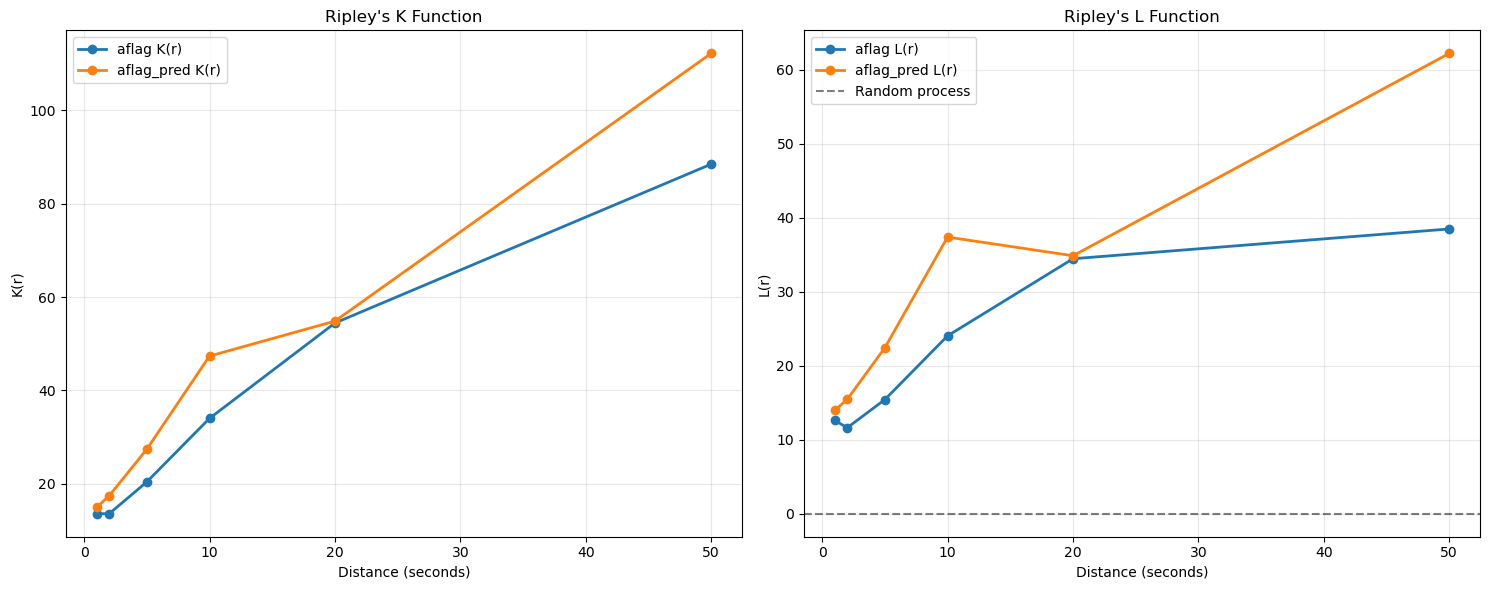
\includegraphics[width=0.9\linewidth]{figures/RIPLEY_181330.png}
    \caption{Ripley's K and L functions comparing ground truth and predicted aggressive trades.}
    \label{fig:ripley-kl}
\end{figure}

\begin{table}[H]
    \centering
    \caption{Ripley's L Function Summary}
    \label{tb:ripley-l}
    \begin{tabular}{lcc}
    \toprule
    \textbf{Metric} & \textbf{AFLAG (True)} & \textbf{AFLAG\_PRED (Predicted)} \\
    \midrule
    Number of Events & 23 & 38 \\
    Event Intensity (events/sec) & 0.0128 & 0.0211 \\
    Average \( L(r) \) & 22.76 & 31.04 \\
    \( L(1s) \) & 12.61 & 13.96 \\
    \( L(2s) \) & 11.61 & 15.45 \\
    \( L(5s) \) & 15.42 & 22.42 \\
    \bottomrule
    \end{tabular}
\end{table}



%----------------------ACF--------------------
We analyze the autocorrelation structure of both the actual and predicted aggressive trade series to assess whether the neural Hawkes process preserves the temporal dependence between trades. The Autocorrelation Function (ACF) and Partial Autocorrelation Function (PACF) plots are shown in Figure~\ref{fig:acf-pacf}, with values interpreted below.

For the actual aggressive trade series (AFLAG), the lag-1 autocorrelation is 0.0842, showing weak but positive short-term dependence. The values quickly drop near zero at higher lags, with lag-5 and lag-10 both being -0.0030. In total, 6 lags are statistically significant, and the Ljung-Box test p-value is essentially zero. This indicates that even though the autocorrelations are small, the process does have significant temporal structure.

For the predicted series (AFLAG\_PRED), the lag-1 autocorrelation is 0.0744, which is very close to the actual series. Lag-5 and lag-10 values are -0.0049, also similar to the actual values. There are 4 significant lags, and the Ljung-Box test again returns a p-value of 0.000000, confirming the presence of temporal dependence.

These results suggest that the neural Hawkes process does not simply generate random aggressive trades, but produces a time series with similar short-term dependency structure as the actual data.

\textbf{Cross-correlation Analysis:} The cross-correlation between the true and predicted series is also computed. The maximum cross-correlation value is 0.0980, occurring at lag 49. The zero-lag correlation is 0.0301. Although the absolute correlation is small, this shows that the predicted sequence partially aligns with the actual series, especially with a slight time shift.

Overall, both the autocorrelation and cross-correlation results support that the neural Hawkes process is capable of capturing temporal structure in aggressive trade patterns.

\begin{figure}[H]
    \centering
    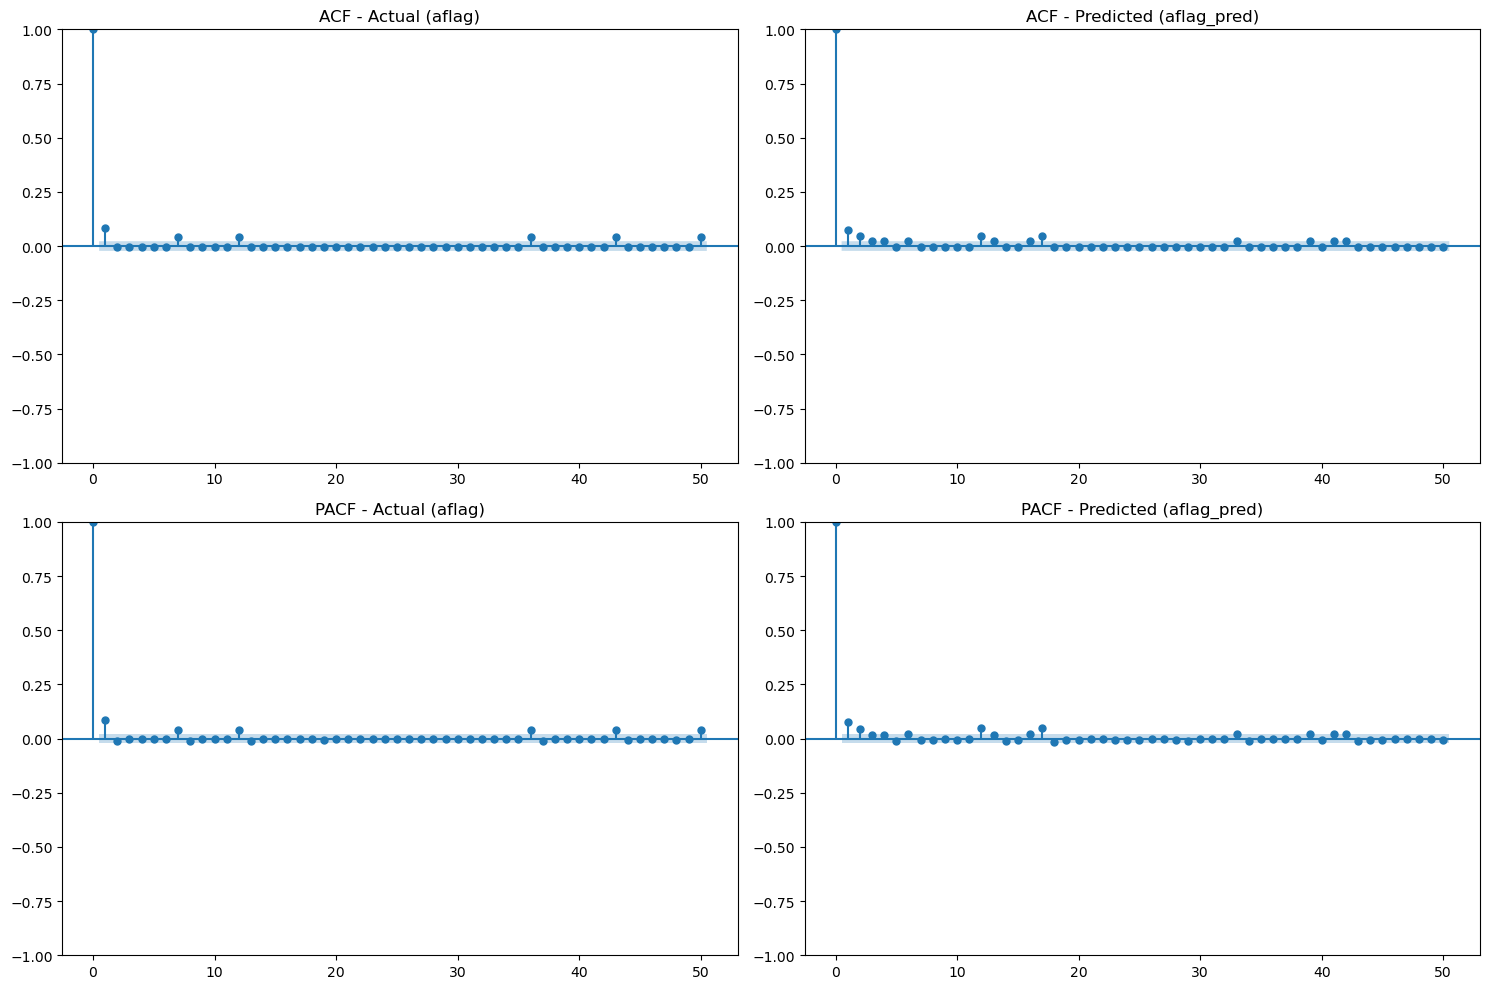
\includegraphics[width=0.95\linewidth]{figures/ACF_181330.png}
    \caption{Autocorrelation (ACF) and Partial Autocorrelation (PACF) plots of actual and predicted aggressive trade series.}
    \label{fig:acf-pacf}
\end{figure}

To evaluate how well the predicted aggressive trade events match the statistical distribution of actual trades, we perform two distributional tests: the Kolmogorov-Smirnov (KS) test and the Kullback-Leibler (KL) divergence.

%----------------Distributional Test-------------
\vspace{0.5em}
\noindent\textbf{Kolmogorov-Smirnov Test:} \\
The KS test is used to compare the cumulative distributions of two sample sets. It returns a test statistic and a p-value. If the p-value is below 0.05, the distributions are considered significantly different.

In our case, the KS statistic is 0.0019 and the p-value is 1.0000, indicating that there is no statistically significant difference between the predicted and actual event distributions. The actual proportion of aggressive trades is 0.0030, and the predicted proportion is 0.0049. The difference between them is only 0.0019. This result shows that the neural Hawkes model accurately matches the distribution of aggressive trade occurrence over time.
\begin{table}[H]
    \centering
    \caption{Kolmogorov--Smirnov Test Results}
    \label{tb:ks-test}
    \begin{tabular}{lr}
    \toprule
    \textbf{Metric} & \textbf{Value} \\
    \midrule
    KS Statistic & 0.0019 \\
    p-value & 1.0000 \\
    Significant (p < 0.05) & False \\
    Actual Proportion & 0.0030 \\
    Predicted Proportion & 0.0049 \\
    Proportion Difference & 0.0019 \\
    \bottomrule
    \end{tabular}
\end{table}

\vspace{0.5em}
\noindent\textbf{Kullback-Leibler Divergence:} \\
KL divergence is a measure of how one probability distribution differs from another. We compute the KL divergence in both directions between the windowed count distributions of the predicted and actual events. 

The value of KL(actual $\parallel$ predicted) is 7.7609 bits, while KL(predicted $\parallel$ actual) is 2.6656 bits. The symmetric KL divergence is 5.2132 bits. These values are relatively moderate, indicating that the predicted distribution is somewhat more peaked or uneven than the actual one. Still, the predicted distribution resembles the actual distribution well enough for backtesting purposes. Lower KL divergence values generally mean higher similarity, and in our case the distributional shape is captured to a reasonable degree.

\begin{figure}[H]
    \centering
    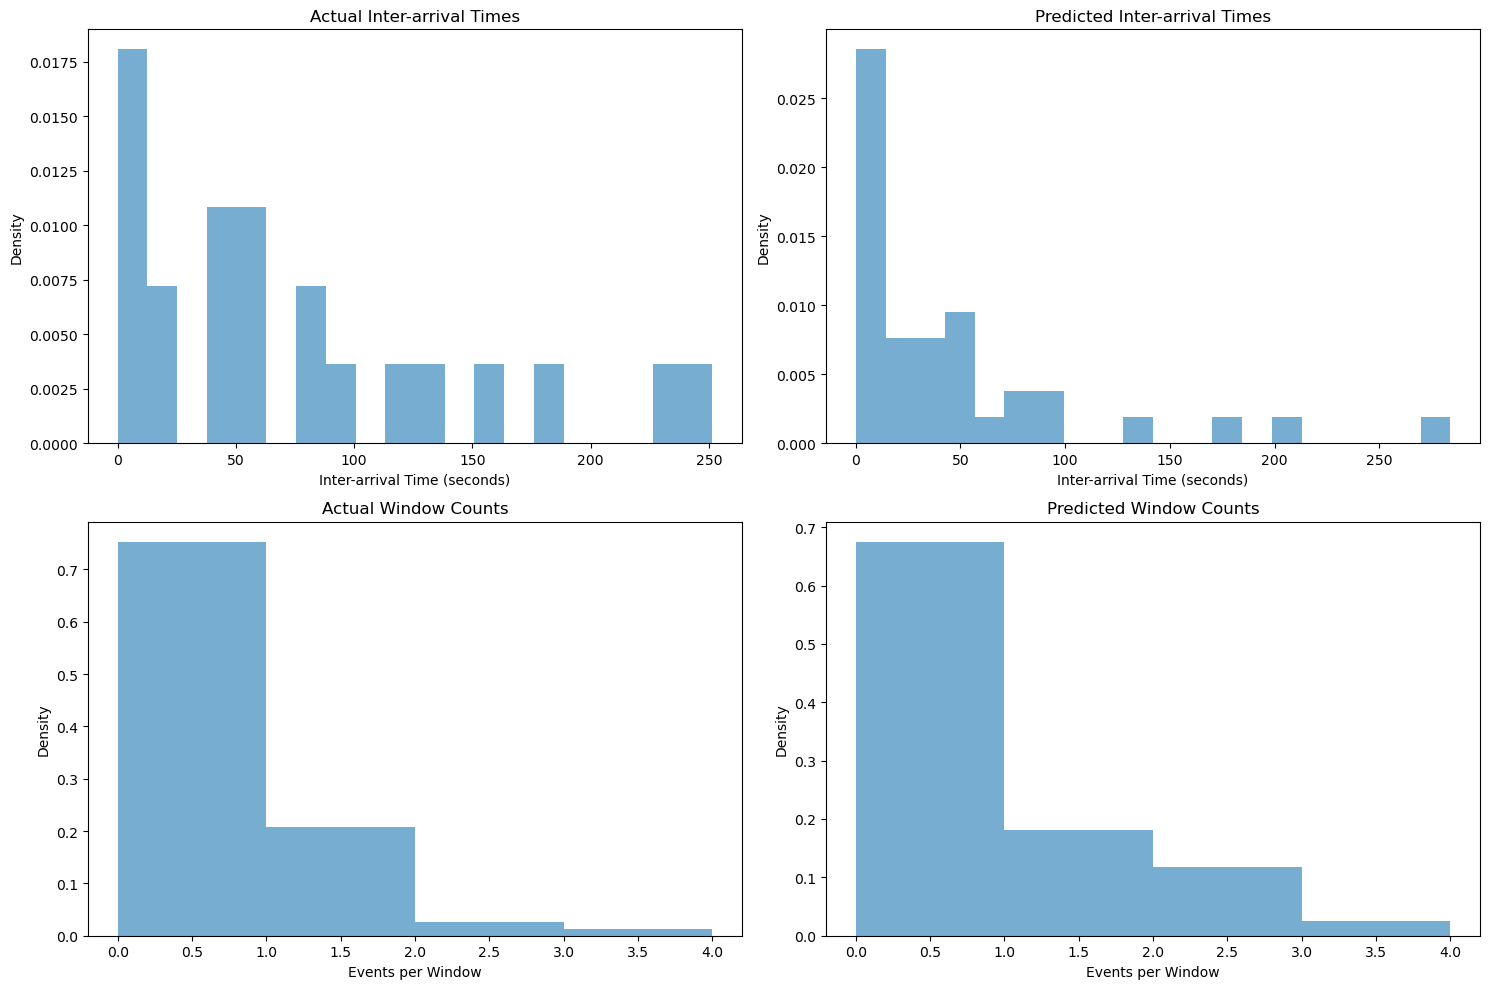
\includegraphics[width=0.95\linewidth]{figures/KL_181330.png}
    \caption{KL divergence plot for event count distributions (predicted vs actual).}
    \label{fig:kl-divergence}
\end{figure}

\begin{table}[H]
    \centering
    \caption{Kullback--Leibler Divergence Between Actual and Predicted Distributions}
    \label{tb:kl-divergence}
    \begin{tabular}{lr}
    \toprule
    \textbf{Metric} & \textbf{Value (bits)} \\
    \midrule
    KL(actual $\parallel$ predicted) & 7.7609 \\
    KL(predicted $\parallel$ actual) & 2.6656 \\
    Symmetric KL Divergence & 5.2132 \\
    \bottomrule
    \end{tabular}
\end{table}


%---------conclusion-----------
Overall, these tests confirm that the neural Hawkes process not only models the timing and clustering of events, but also captures the underlying distributional structure of aggressive trade frequency.

The Neural Hawkes Process with GRU kernel captures meaningful patterns in trade timing. It shows interpretable dynamics like short-term excitation, quick decay, and clustering, especially for aggressive trades. This supports our idea that using intensity-based simulation gives us more insight and control than pure black-box classifiers.









\subsection{Result Conclusion and Data Flow}
\begin{figure}[H]
    \centering
    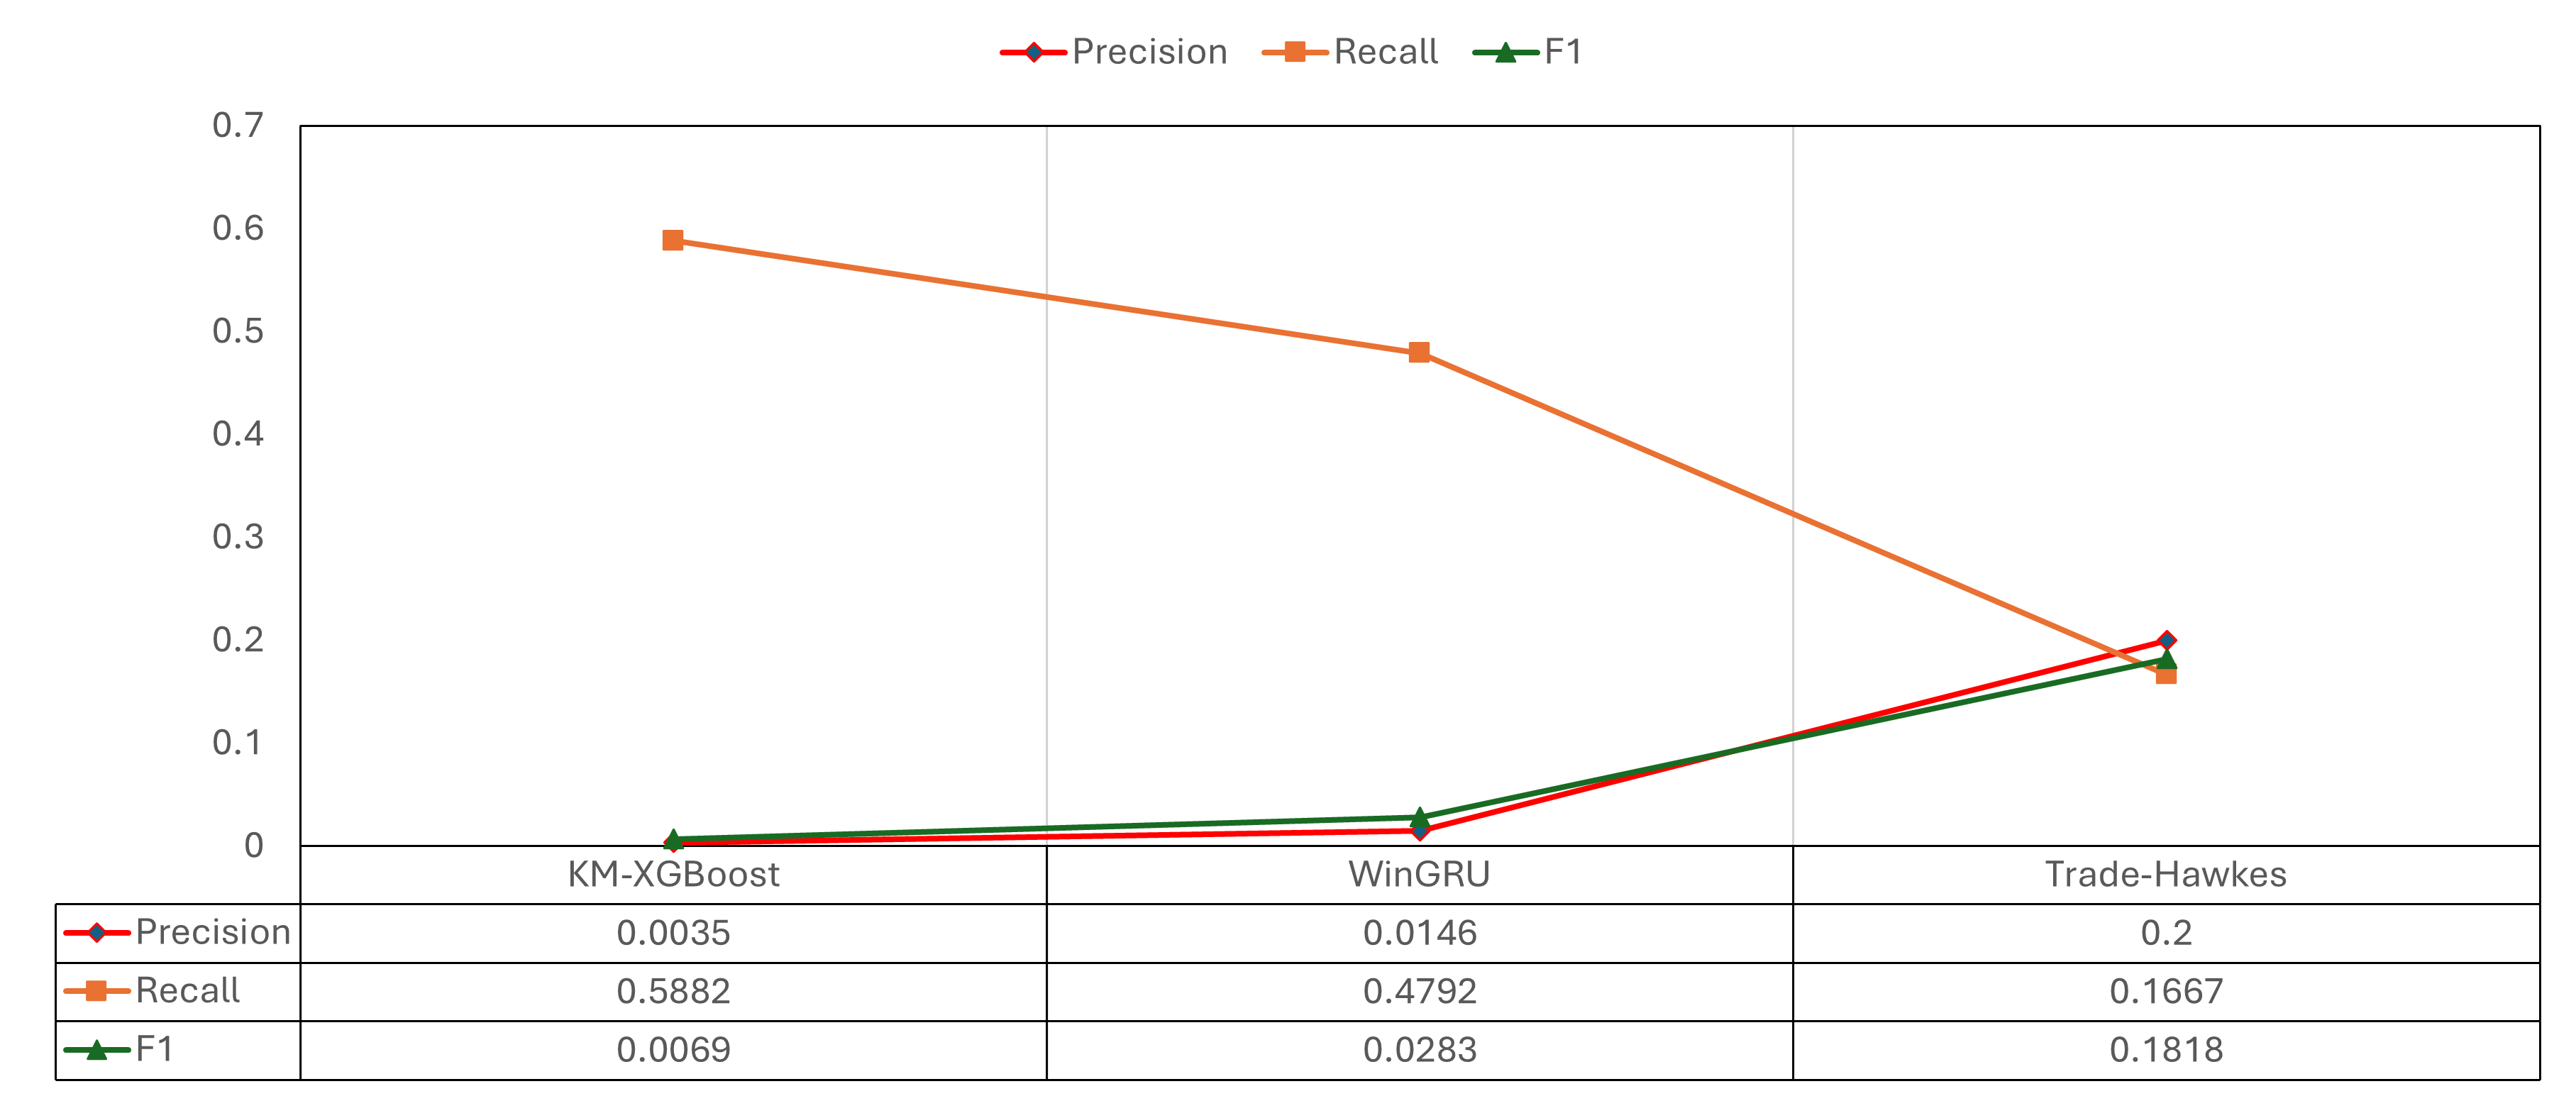
\includegraphics[width=0.9\textwidth]{figures/final_performance_plot.png}
    \caption{Precision, recall, and F1-score across different stages.}
    \label{fig:final-performance}
\end{figure}

\begin{figure}[H]
    \centering
    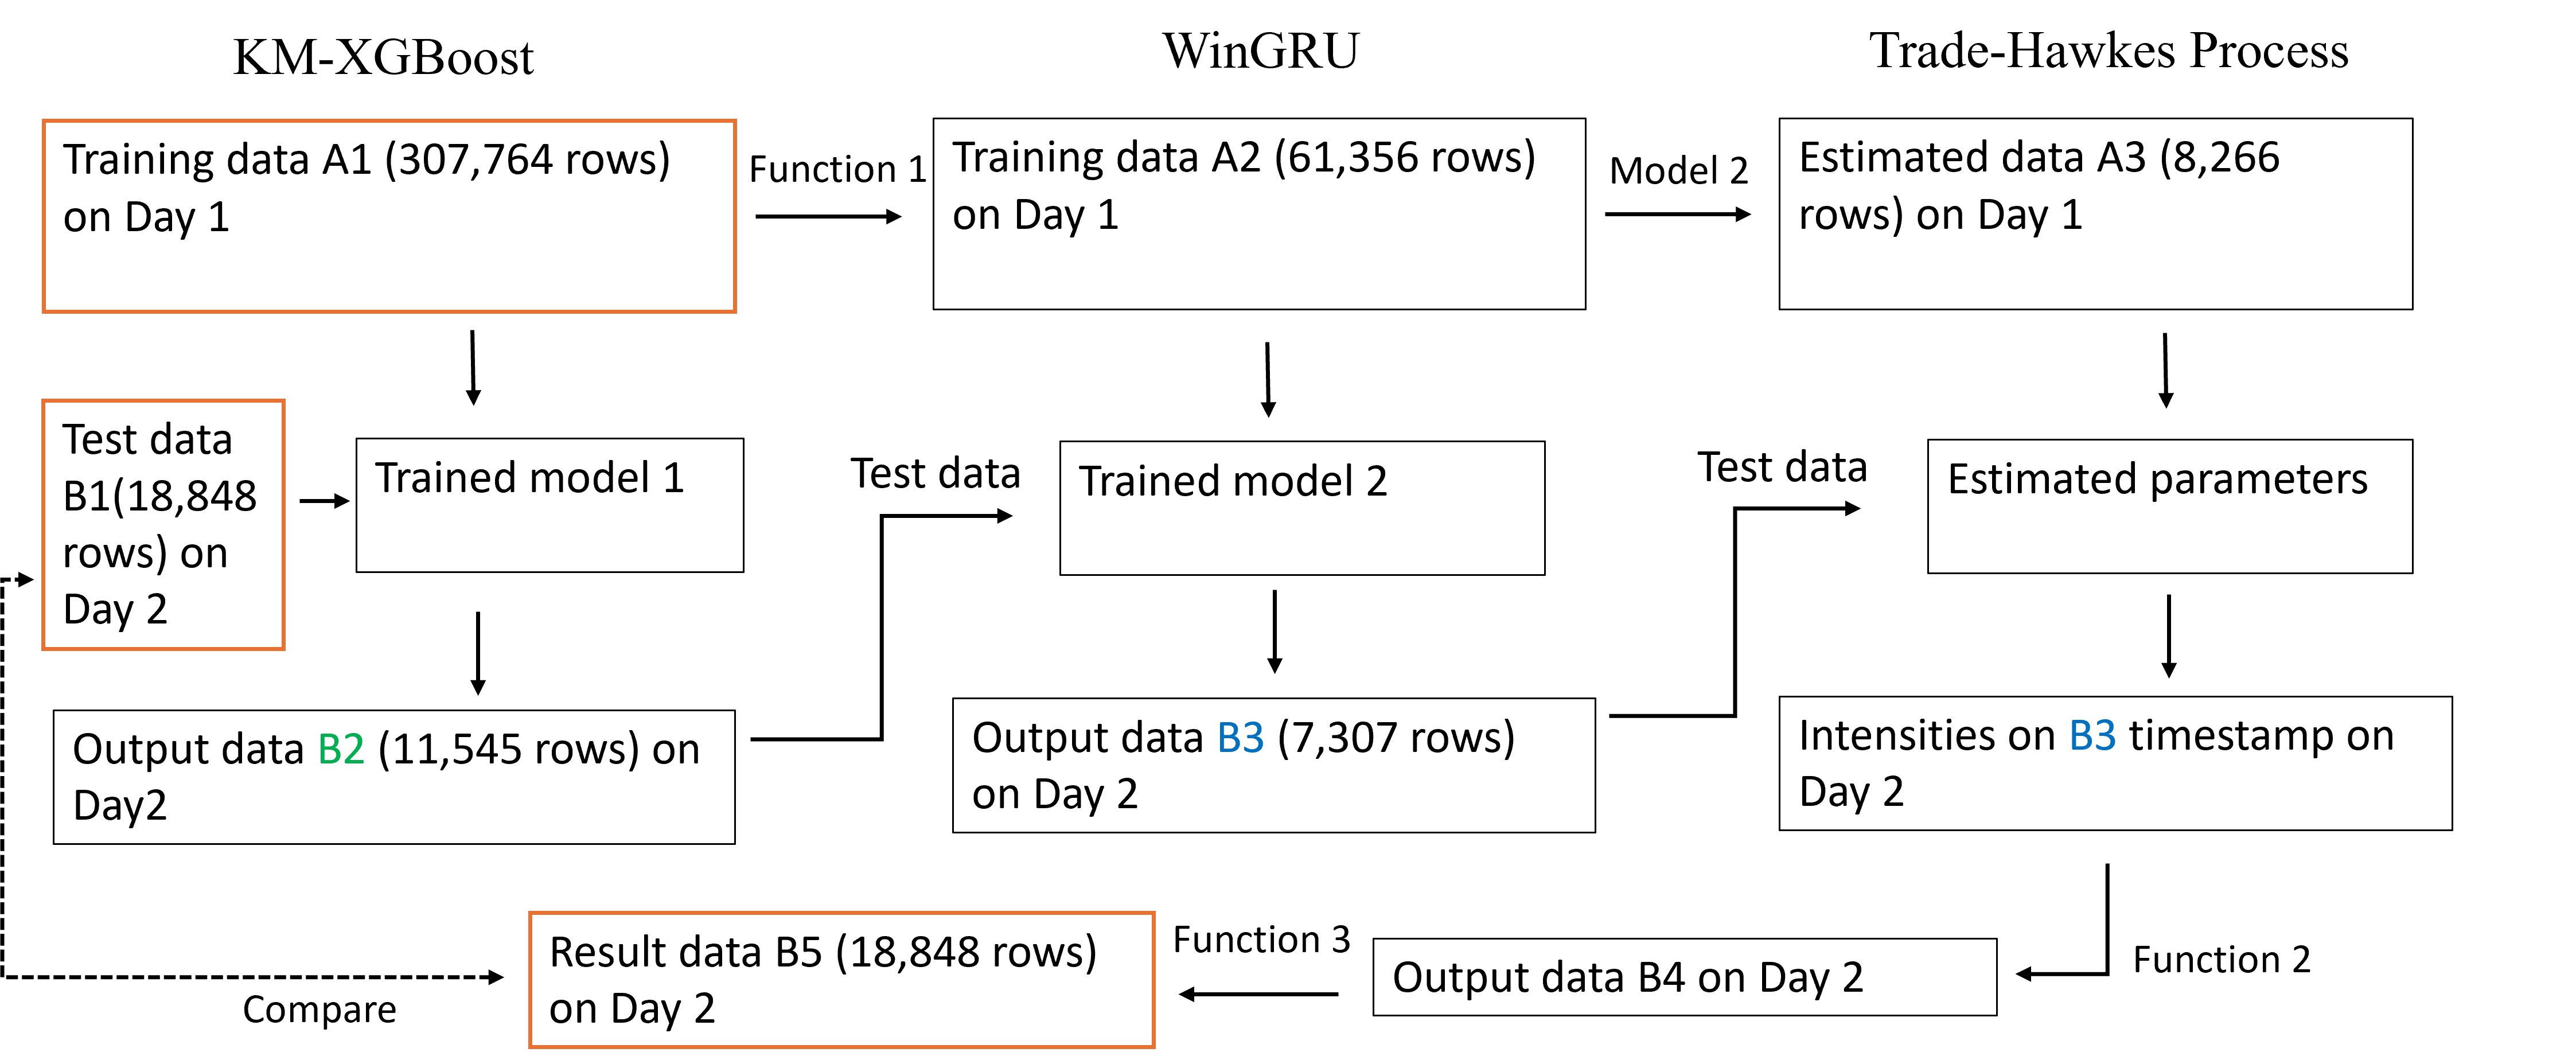
\includegraphics[width=\textwidth]{figures/data flow.png}
    \caption{Data flow of the full pipeline from raw data to final prediction.}
    \label{fig:data-flow-diagram}
\end{figure}




\section{Prediction Performance}
In this section, we evaluate the performance of the Two-stage Machine Learning and Stochastic Modeling Framework on different trading days, including. The results are compared against several single-model benchmark models, such as only XGBoost, only GRU and Hawkes process. This comparison demonstrates the accuracy and effectiveness of the combined framework in improving simulation performance, particularly under extreme class imbalance.













% \section{Prediction for $\bar{\alpha}$}
% \begin{figure}[h]
%     \centering
%     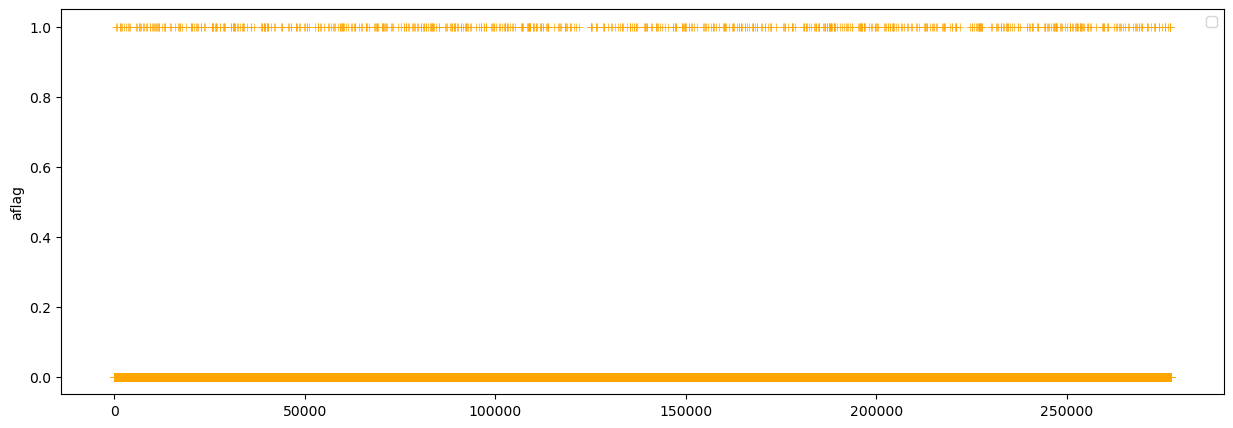
\includegraphics[width=\linewidth]{figures/aflag.png}
%     \caption{Binary distribution of the aggressive trade flag $\bar{\alpha}$}
%     \label{fig: aflag}
%     {\small \textit{Note.} Each point with value 1 indicates the occurrence of an aggressive trade, while 0 indicates non-aggressive or no trade.}
% \end{figure}
% Figure.~\ref{fig: aflag_class_distribution} shows $\bar{\alpha}$ faces severe class imbalance, which can lead to biased model predictions if not addressed. Class 0 dominates the dataset, accounting for 99.8\% of all samples, while Class 1 accounts for only 0.2\%. To solve this imbalance, techniques such as resampling, weighted loss functions, and anomaly detection methods are employed. 
% \begin{figure}[h]
%     \centering
%     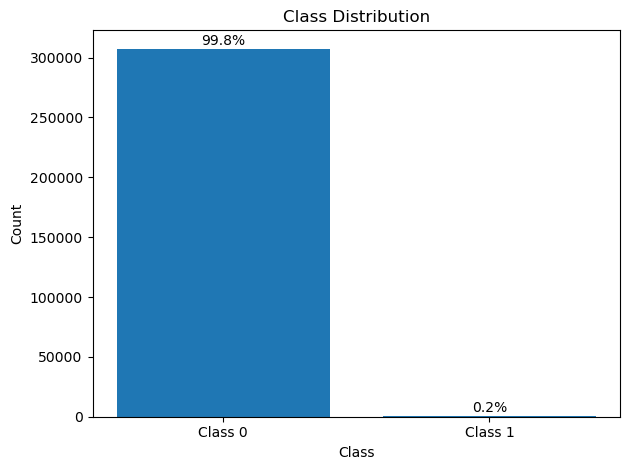
\includegraphics[width=0.8\linewidth]{figures/Imbalaced data for aflag.png}
%     \caption{Class Distribution for $\bar{\alpha}$}
%     {\small \textit{Note.} In the overall 308,178 data, class 0 accounts for 99.8\% of the samples, while Class 1 represents only 0.2\%, indicating a severe class imbalance.}
%     \label{fig: aflag_class_distribution}
% \end{figure}
% \newpage
% \subsection{XGBoost}
% \begin{figure}[h]
%     \centering
%     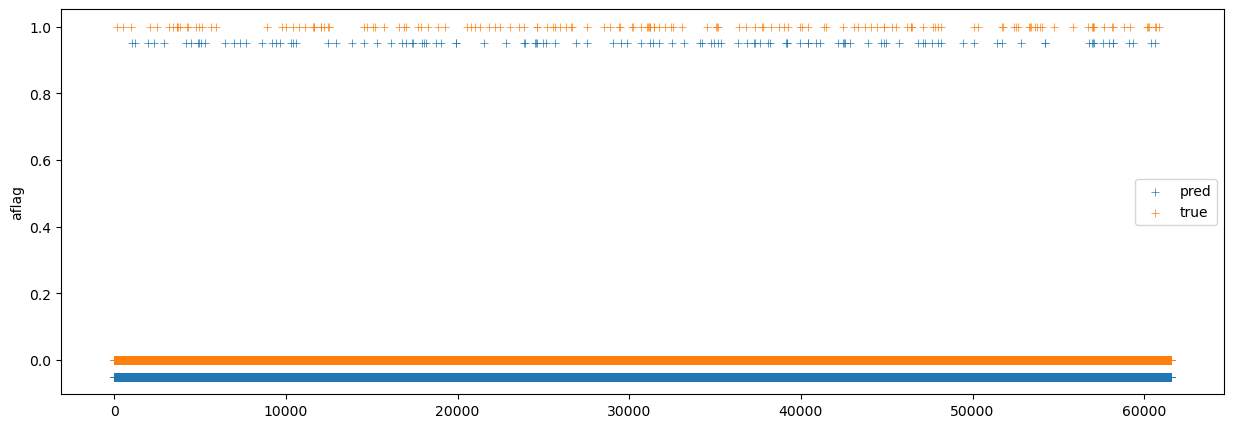
\includegraphics[width=\linewidth]{figures/aflag_XGBoost.png}
%     \caption{Predicted and true values of $\bar{\alpha}$}
%     \label{fig:aggressive_flag_prediction}
%     {\small \textit{Note.} The plot compares the predicted and true values of the aggressive flag. Each `+` marker represents a positive prediction (blue) or ground truth (orange). The strong class imbalance and sparsity of positive cases make correct prediction more difficult, highlighting the challenge of this classification task.}
% \end{figure}
% The model's performance on the test set is summarized by the confusion matrix and associated classification metrics. 

% \begin{table}[h]
% \centering
% \caption{Confusion Matrix}
% \begin{tabular}{c|cc}
% \toprule
%               & Predicted 0 & Predicted 1 \\
% \midrule
% Actual 0      & 61311       & 99          \\
% Actual 1      & 136         & 17          \\
% \bottomrule
% \end{tabular}
% \label{tab:confusion_matrix}
% \vspace{2mm}

% {\small \textit{Note.} The confusion matrix shows a strong true negative rate but a weak true positive rate, which is expected in highly imbalanced classification tasks.}
% \end{table}

% \begin{table}[h]
% \centering
% \caption{Classification Report}
% \begin{tabular}{lcccc}
% \toprule
% Class & Precision & Recall & F1-score & Support \\
% \midrule
% 0     & 0.9978    & 0.9984 & 0.9981   & 61410   \\
% 1     & 0.1466    & 0.1111 & 0.1264   & 153     \\
% \midrule
% Accuracy     & \multicolumn{3}{c}{0.9962} & 61563 \\
% Macro Avg    & 0.5722 & 0.5547 & 0.5622   & 61563 \\
% Weighted Avg & 0.9957 & 0.9962 & 0.9959   & 61563 \\
% \bottomrule
% \end{tabular}
% \label{tab:classification_report}
% \vspace{2mm}

% {\small \textit{Note.} While the overall accuracy is high due to the dominance of class 0, the metrics for class 1 reveal the difficulty of detecting aggressive trades.}
% \end{table}

% \noindent
% \textbf{AUC:} 0.6424
% {\small \textit{Note.} The Area Under the Curve (AUC) score indicates the ability to separate the two classes.}

% \subsection{Feature Importance}
% \begin{figure}[h]
%     \centering
%     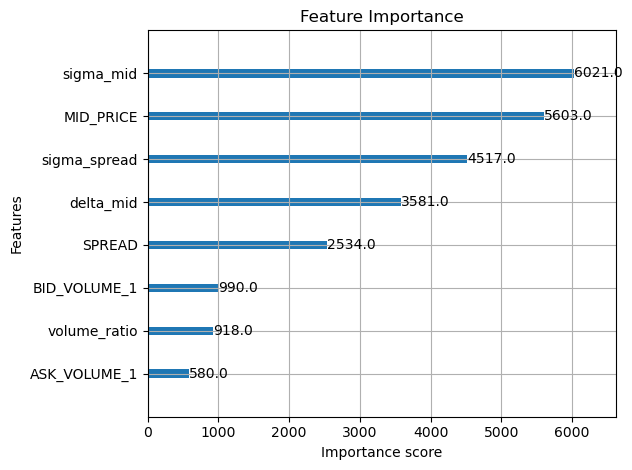
\includegraphics[width=\linewidth]{figures/feature importance.png}
%     \caption{Feature importance scores for predicting aggressive trades}
%     \label{fig:feature_importance_af}
%     {\small \textit{Note.} The most important features include \texttt{sigma\_mid}, \texttt{MID\_PRICE}, and \texttt{sigma\_spread}, indicating that mid-price volatility and spread dynamics play a key role in identifying aggressive trade behavior. Volume-related features such as \texttt{ASK\_VOLUME\_1} and \texttt{BID\_VOLUME\_1} are less influential.}
% \end{figure}

% \newpage


% \section{Prediction for $\alpha$}
% \begin{figure}[h]
%     \centering
%     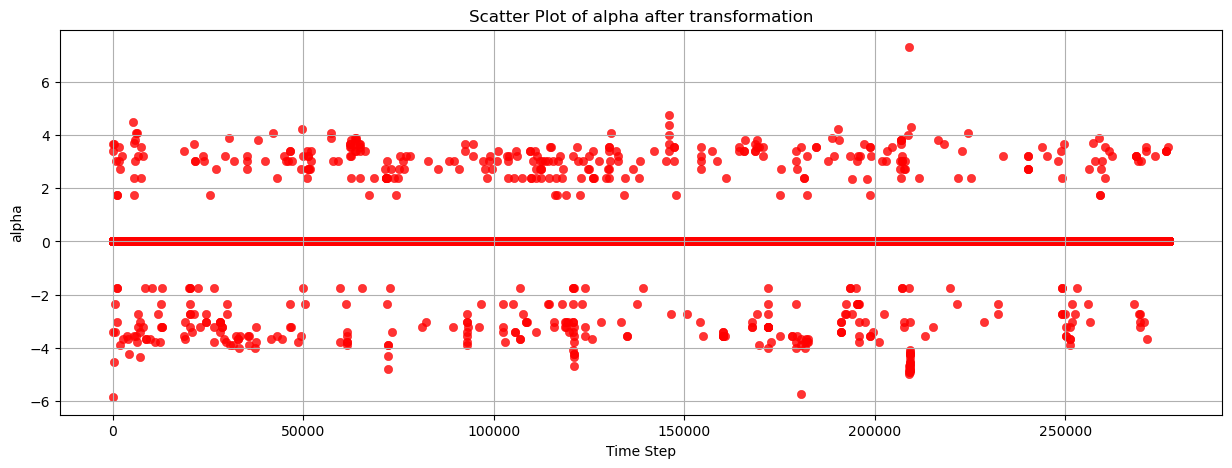
\includegraphics[width=\linewidth]{figures/alpha after transformation.png}
%     \caption{Scatter plot of transformed $\alpha$ values over time}
%     \label{fig:alpha_transformed_scatter}
%     {\small \textit{Note.} This plot visualizes the transformed $\alpha$ signal across time steps. Most values are concentrated near zero, while some are clearly positive or negative.}
% \end{figure}
% \subsection{GRU-based Neural Network}
% \begin{figure}[h]
%     \centering
%     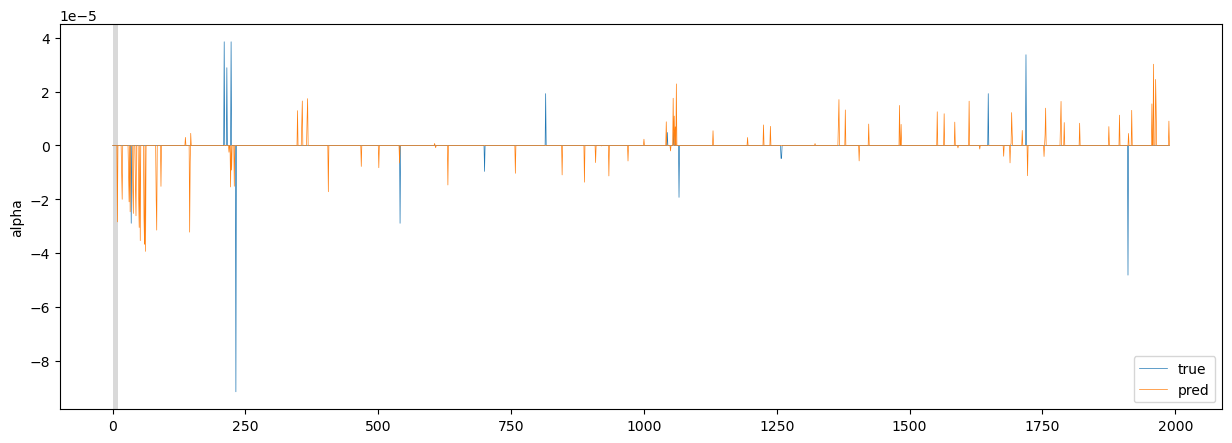
\includegraphics[width=\linewidth]{figures/alpha_GRU.png}
%     \caption{Prediction of $\alpha$ using a GRU-based model}
%     \label{fig:gru_alpha_prediction}
%     {\small \textit{Note.} This plot compares the predicted $\alpha$ values from a GRU model (orange) against the ground truth (blue). The GRU captures some local patterns.}
% \end{figure}
% \begin{figure}[h]
%     \centering
%     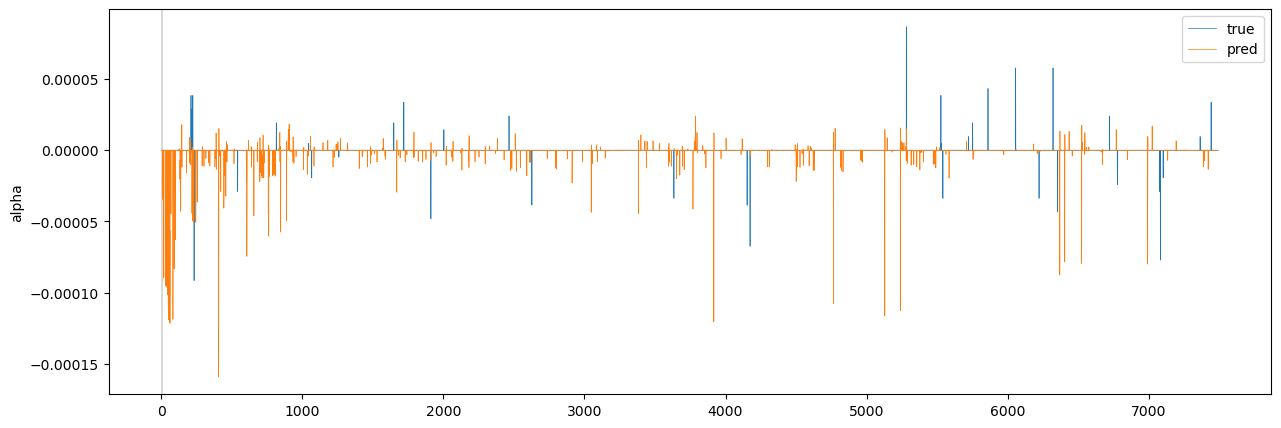
\includegraphics[width=\linewidth]{figures/alpha_Linear.png}
%     \caption{Prediction of $\alpha$ using a linear regression model}
%     \label{fig:lr_alpha_prediction}
%     {\small \textit{Note.} The linear regression model shows limited ability to capture fluctuations in $\alpha$, often underestimating both amplitude and timing compared to the true values. This highlights the limitations of linear models in capturing non-linear temporal dependencies.}
% \end{figure}

% \begin{table}[h]
%     \centering
%     \caption{Performance comparison between GRU and Linear Regression for $\alpha$ prediction}
%     \label{tab:gru_vs_lr}
%     \begin{tabular}{lcc}
%         \toprule
%         Metric & GRU & Linear Regression \\
%         \midrule
%         MSE   & 0.1348  & 0.3336 \\
%         RMSE  & 0.3672  & 0.5776 \\
%         MAE   & 0.0263  & 0.0367 \\
%         %R$^2$ & 3.1362  & 21.0387 \\
%         MAPE (\%) & 63.47  & 62.74 \\
%         SMAPE (\%) & 59.95  & 62.11 \\
%         \bottomrule
%     \end{tabular}
% \end{table}
% Table~\ref{tab:gru_vs_lr} compares the performance of the GRU model and the linear regression model on the task of predicting $\alpha$. The GRU model achieves lower MSE (0.1348 vs. 0.3336), RMSE (0.3672 vs. 0.5776), and MAE (0.0263 vs. 0.0367), indicating better overall prediction accuracy. Although both models show similar MAPE and SMAPE values, the GRU produces a slightly lower symmetric error. 
% % The R$^2$ values are unusually high for both models, likely due to the small magnitude of $\alpha$ and possible data scaling effects, but the relative comparison still shows the GRU outperforming the linear model. 
% Overall, the GRU model demonstrates better capability in capturing the temporal and nonlinear dynamics of the data.

% \section{Prediction for $\tau$}
% Figure.~\ref{fig: Countdown} shows how much time is left until the next aggressive trade. Each point at 0 represents for an aggressive trade. After each zero point, a sharp increase marks the start of a new countdown period leading up to the next aggressive trade.
% \begin{figure}[h]
%     \centering
%     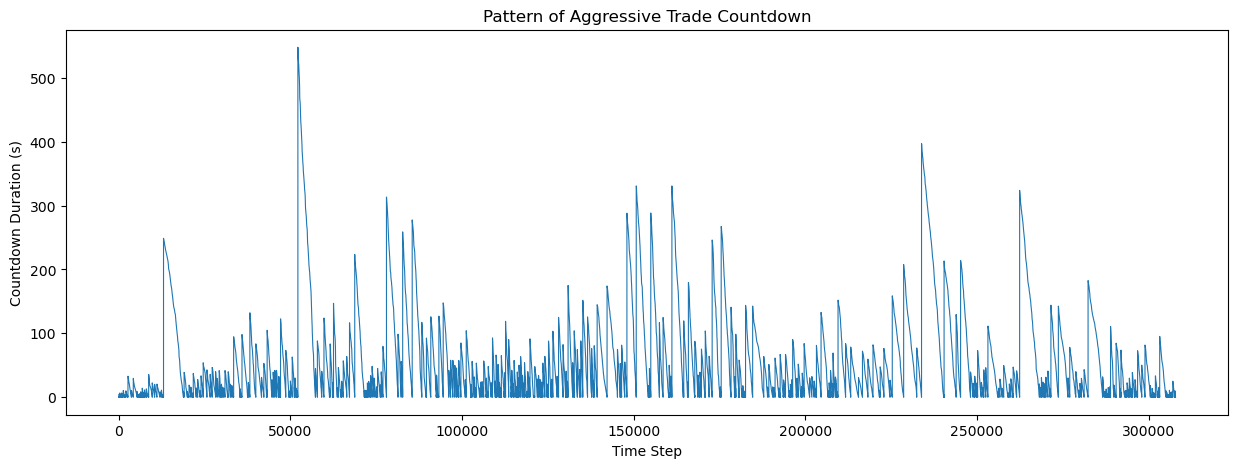
\includegraphics[width=\linewidth]{figures/Pattern of Aggressive Trade Countdown.png}
%     \caption{Countdown to the next aggressive trade}
%     \label{fig: Countdown}
% \end{figure}

% \subsection{XGBoost}
% \subsection{Recurrent Neural Networks}
% The feature matrix $X$ and the target vector $y$ are converted to NumPy arrays. The dataset is split into training (90\%) and testing (10\%) sets. Both the input and output are scaled to improve convergence during training. Inputs are normalized to the range $[0, 1]$ using a MinMaxScaler. For the output, to enhance the sensitivity of the model to small but informative signals, we applied a signed logarithmic transformation to selected features. The transformation preserves the original sign of the data, compresses large magnitudes, and expands small nonzero values, making subtle patterns more noticeable to the model. After applying the logarithmic adjustment, the transformed values are rescaled to fit within the range \([-1, 1]\). An inverse transformation is also defined to recover the original values when necessary, maintaining consistency between the transformed and original feature spaces.


% \section{Ablation Studies}
% Impact of different model components (CGAN vs. pure Hawkes vs. hybrid). Sensitivity analysis on model hyperparameters.


% \section{Backtesting Performance}
% Simulating market impact with aggressive/passive execution strategies.
% Evaluating execution cost and slippage in various market scenarios.
% Comparing execution performance with traditional historical replay.

% \section{Application to other products}
% other products, like FX options, equity...